
% This LaTeX was auto-generated from MATLAB code.
% To make changes, update the MATLAB code and republish this document.

\documentclass{article}
\usepackage{graphicx}
\usepackage{color}

\sloppy
\definecolor{lightgray}{gray}{0.5}
\setlength{\parindent}{0pt}

\begin{document}

    
    
\section*{Reguleringsteknikk eksamen}


\subsection*{Contents}

\begin{itemize}
\setlength{\itemsep}{-1ex}
   \item Task 1
   \item a) State-space representation
   \item State Space Representation
   \item b) simulink implementations
   \item c) PID design
   \item c/d) Applying the control to the non-linear and linearized plants in simulink
   \item Task 2
   \item a) poles and zeros
   \item b) Step response
   \item c) Stability
   \item d) P-control equivalent transfer function
   \item e) Kp-stable values
   \item f/g/h)
   \item i)
   \item Task 3
   \item a/b) System transfer functions
   \item c) Plant step response
   \item d) poles
   \item f) new A matrix
   \item g) step responses
\end{itemize}


\subsection*{Task 1}



\subsection*{a) State-space representation}

\begin{par}
Differential equation describing the tank water level:
\end{par} \vspace{1em}
\begin{par}
$$ \frac{d}{dt}H = \frac{bV-a\sqrt{H}}{A} $$
\end{par} \vspace{1em}
\begin{par}
This ode is non-linear in $\sqrt{H}$. However, we can approximate this by a first order taylor expansion/linearization in a neighbourhood $H_0 + \hat{H}$ around the stationary point $H_0$:
\end{par} \vspace{1em}
\begin{par}
$$ \sqrt{H_0 + \hat{H}} \approx \sqrt{H_0} + \frac{1}{2\sqrt{H_0}}\cdot (H-H_o) $$
\end{par} \vspace{1em}
\begin{par}
With this linearization we arrive at the linear ODE:
\end{par} \vspace{1em}
\begin{par}
$$ \frac{dH}{dt} =\frac{b}{A} V - \frac{a}{2A} \sqrt{H_0} (H-H_0) - \frac{a\sqrt{H_0}}{A} $$
\end{par} \vspace{1em}


\subsection*{State Space Representation}

\begin{par}
We can find the state space representation of this system (ignoring the non-homogeneous part):
\end{par} \vspace{1em}
\begin{par}
$$ \frac{d}{dt} H = \left[\matrix{ - \frac{a}{2A \sqrt{H_0}}} \right] H + \left[\matrix{ \frac{b}{A}} \right]V $$
\end{par} \vspace{1em}
\begin{par}
Alternatively, with our constants and linearization point:
\end{par} \vspace{1em}
\begin{par}
$$ \dot{H} = \left[\matrix{ - \frac{3\sqrt{10}}{80}} \right] H + \left[\matrix{ \frac{1}{3}} \right]V $$
\end{par} \vspace{1em}
\begin{par}
Our state space consists of a one-dimensional state vector H and a one-dimensional control vector V
\end{par} \vspace{1em}


\subsection*{b) simulink implementations}

\begin{par}
Open-loop non-linear system:
\end{par} \vspace{1em}
\begin{par}

\includegraphics [width=4in]{open_loop_nonlinear.png}

\end{par} \vspace{1em}
\begin{par}
Open-loop linear system:
\end{par} \vspace{1em}
\begin{par}

\includegraphics [width=4in]{open_loop_linear.png}

\end{par} \vspace{1em}


\subsection*{c) PID design}

\begin{par}
Now we develop a complete PID controller for our plant using the transfer function of the linearized model.
\end{par} \vspace{1em}
\begin{verbatim}
close;
s = tf('s');

A = 24; b = 8; a = 18; %water tank parameters
tf_linear = (b/A)/(s+1/(2*sqrt(10))*(a/A)); %defining transfer function as given in the task
step(tf_linear);
\end{verbatim}

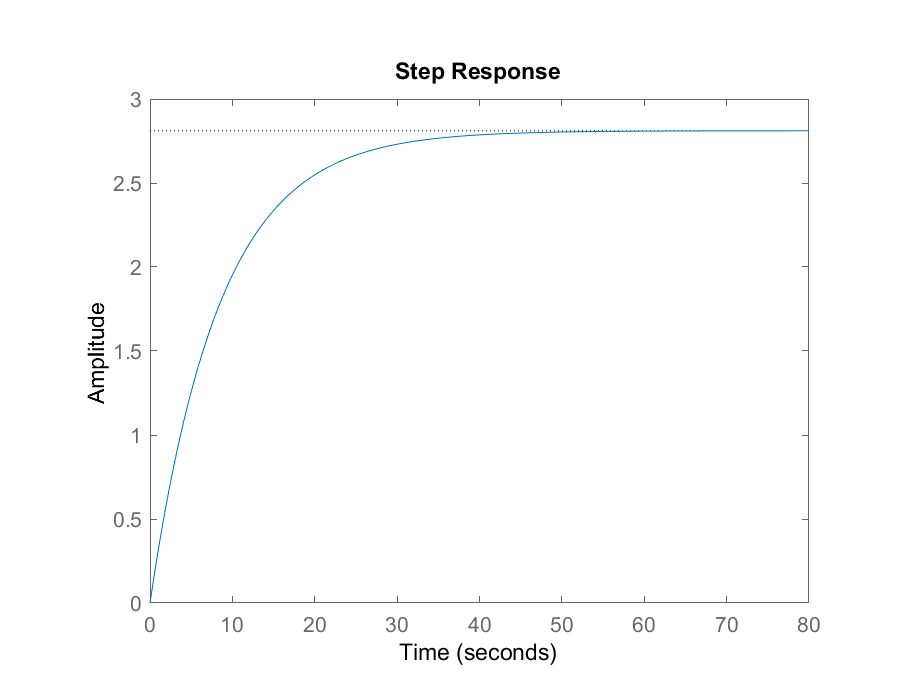
\includegraphics [width=4in]{main_01.eps}
\begin{par}
Now we tune all the gains to achieve the desired response
\end{par} \vspace{1em}
\begin{verbatim}
Kp = 15;
Ki = 5;
Kd = 1;

H = tf_linear; %plant transfer function
C = Kp + Ki/s + Kd*s; %PID transfer function

CH = C*H; %closed loop transfer function
closed_tf = CH/(CH+1);
step(closed_tf);

info = stepinfo(closed_tf);
overshoot     = info.Overshoot;
rise_time     = info.RiseTime;
settling_time = info.SettlingTime;

% Display results
fprintf('Overshoot: %.2f%%\n', overshoot);
fprintf('Rise Time: %.2f s\n', rise_time);
fprintf('Settling Time: %.2f s\n', settling_time);
grid on;
\end{verbatim}

        \color{lightgray} \begin{verbatim}Overshoot: 2.95%
Rise Time: 0.51 s
Settling Time: 3.76 s
\end{verbatim} \color{black}
    
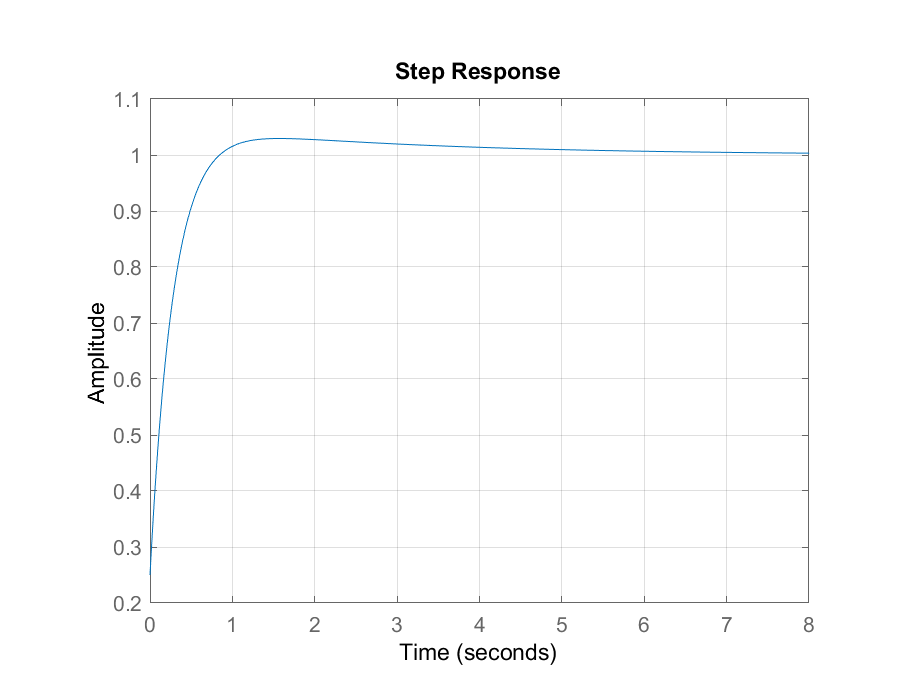
\includegraphics [width=4in]{main_02.eps}


\subsection*{c/d) Applying the control to the non-linear and linearized plants in simulink}

\begin{par}
With our conservative gains [Kp, Ki, Kd] = [15, 5, 1] We achieved a nice response.
\end{par} \vspace{1em}
\begin{par}
Here I plot the response for a setpoint of 10 an an initial tank level of 9, for both the non-linear and linear systems.
\end{par} \vspace{1em}
\begin{par}

\includegraphics [width=4in]{high_level_closed_loop.png}

\end{par} \vspace{1em}
\begin{par}

\includegraphics [width=4in]{closed_loop_response.png}

\end{par} \vspace{1em}
\begin{par}
The response of the linear system here is not just a scaled version of the closed\_loop unit step response, since the setpoint and initial conditions arent just scaled versions of the unit step (theres a translation in the setpoint). If we instead  plotted the response of a setpoint of 10 and an initial condition of 0, the response of the linearized system would be identical to a scaled version of the unit step response.
\end{par} \vspace{1em}
\begin{verbatim}
% We also see again that the linear approximation starts out good, but diverges from the true state of the system as we get further away from the linearization point.
\end{verbatim}


\subsection*{Task 2}



\subsection*{a) poles and zeros}

\begin{par}
the transfer function, with canard deflection as input and pitch altitude as output, is given as:
\end{par} \vspace{1em}
\begin{par}
$$ \frac{\theta}{\delta_c} = \frac{s+24}{(s-8)(s-18)} $$
\end{par} \vspace{1em}
\begin{par}
This system is clearly unstable, as both poles are positive real numbers (8 and 18). We can verify this by using pzplot and looking at the poles:
\end{par} \vspace{1em}
\begin{verbatim}
s = tf('s');
sys = (s+24)/((s-8)*(s-18));
pzplot(sys);
\end{verbatim}

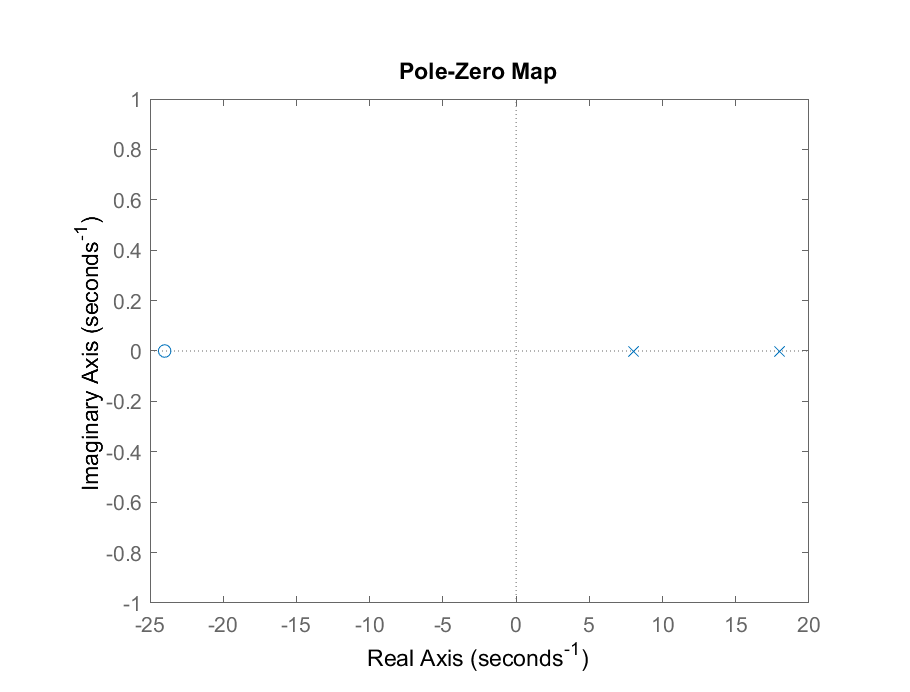
\includegraphics [width=4in]{main_03.eps}


\subsection*{b) Step response}

\begin{verbatim}
close;
step(sys);
\end{verbatim}

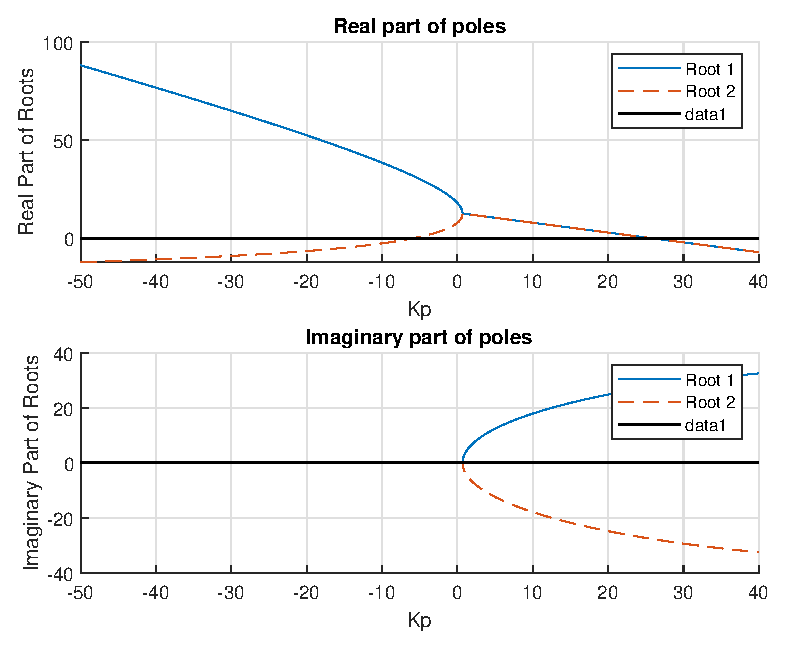
\includegraphics [width=4in]{main_04.eps}


\subsection*{c) Stability}

\begin{par}
The output of our system blows up to infinity, so it is clearly unstable. The open-loop system does not satisfy BIBO, and requires closed loop control to become stable.
\end{par} \vspace{1em}


\subsection*{d) P-control equivalent transfer function}

\begin{par}
We add a proportional control and find an equivalent transfer function for the whole system. I use the simulink block diagram to help find the expression for the new system:
\end{par} \vspace{1em}
\begin{par}

\includegraphics [width=4in]{tf_with_proportional_gain.png}

\end{par} \vspace{1em}
\begin{par}
$$ \theta = K_p \theta_c H(s) - K_p\theta H(s)$$
\end{par} \vspace{1em}
\begin{par}
$$\theta(K_p H(s) + 1) = \theta_c K_p H(s)$$
\end{par} \vspace{1em}
\begin{par}
$$\frac{\theta}{\theta_c} = \frac{K_p H(s)}{K_p H(s) + 1}$$
\end{par} \vspace{1em}
\begin{par}
I insert the plant model $H(s)$ to obtain the full closed loop transfer function:
\end{par} \vspace{1em}
\begin{par}
$$\frac{\theta}{\theta_c} = \frac{K_p \frac{s+24}{s^2-26+144}}{K_p \frac{s+24}{s^2-26+144} + 1} $$
\end{par} \vspace{1em}
\begin{par}
Finally, simplifying the fraction gives:
\end{par} \vspace{1em}
\begin{par}
$$\frac{\theta}{\theta_c} = \frac{K_p s+ K_p 24}{s^2+(K_p-26)s+(144+24K_p)} $$
\end{par} \vspace{1em}


\subsection*{e) Kp-stable values}

\begin{par}
We can show this mathematically by finding the Kp values for which all our poles are in the negative half-plane (negative real part). To do this we look we analyze the denominator of our transfer function with the quadratic formula.
\end{par} \vspace{1em}
\begin{par}
equation:
\end{par} \vspace{1em}
\begin{par}
$$ s^2 + (K_p-26)s+(144+24Kp)= 0$$
\end{par} \vspace{1em}
\begin{par}
We need the real parts of the roots to both be negative. The roots are found by the quadratic equation:
\end{par} \vspace{1em}
\begin{par}
$$ \frac{-(K_p-26)\pm \sqrt{(K_p-26)^2-4(144+24K_p)}}{2} $$
\end{par} \vspace{1em}
\begin{par}
The strictly real part is $\frac{26-K_p}{2}$. If the discriminant $(K_p-26)^2-4(144+24K_p)$ is negative or zero, then the real part is just $\frac{26-K_p}{2}$, and our system is obviously stable for all $K_p > 26$. If the discriminant is positive however, the root will be strictly real, and we need to verify that they are still negative, by checking that
\end{par} \vspace{1em}
\begin{par}
$$-(K_p-26) > \sqrt{(K_p-26)^2-4(144+24K_p)}, \quad \forall K_p > 26  $$
\end{par} \vspace{1em}
\begin{par}
$$(-K_p+26)^2 > (K_p-26)^2-4(14+24K_p)$$
\end{par} \vspace{1em}
\begin{par}
$${K_p}^2-52K_p+26^2 > K_p^2-52K_p+26^2-576-96K_p $$
\end{par} \vspace{1em}
\begin{par}
$$ 96K_p > 576$$
\end{par} \vspace{1em}
\begin{par}
$$ K_p > 6$$
\end{par} \vspace{1em}
\begin{par}
This inequality will obviously also hold for $K_p > 26$. We have now shown that all the roots have negative real parts for all $K_p > 26$, so that our system is stable.
\end{par} \vspace{1em}


\subsection*{f/g/h)}

\begin{par}
For the proportional controller i chose Kp = 147 (see full assignment in attachments):
\end{par} \vspace{1em}
\begin{verbatim}
closed_loop = (Kp*s+Kp*24)/(s^2+(Kp-26)*s+(144+24*Kp));
% We have verified that the poles of our new system are all negative real part. This means the system stable, and we can verify this
% by viewing the step response of the closed loop system:

step(closed_loop)
[y,t]=step(closed_loop); %save the output values to check steady state
SS_error = abs(1-y(end))
%verifying that the new system is stable
isstable(closed_loop)
close;
pzplot(closed_loop)
\end{verbatim}

        \color{lightgray} \begin{verbatim}
SS_error =

   1.2858e+25


ans =

  logical

   0

\end{verbatim} \color{black}
    
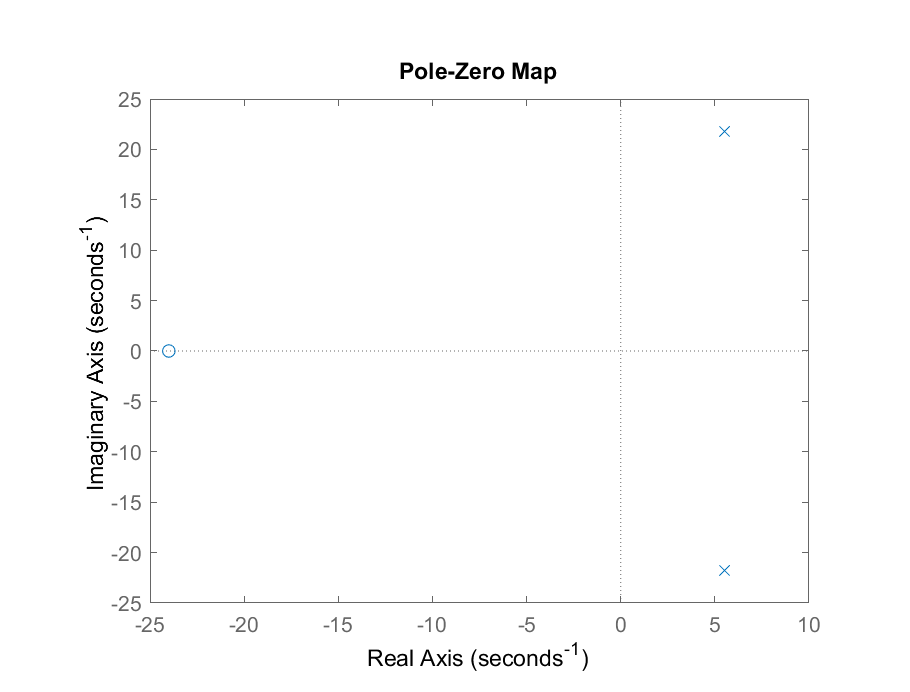
\includegraphics [width=4in]{main_05.eps}
\begin{par}
Thus we have verified that our control system is stable and reaches a steady state error of 3.89\%, with a steady state value of
\end{par} \vspace{1em}
\begin{par}
$$(1-\frac{3.89}{100}) = 0.9611 $$
\end{par} \vspace{1em}


\subsection*{i)}

\begin{par}
The new system is stable, as shown by the poles and step response.
\end{par} \vspace{1em}


\subsection*{Task 3}



\subsection*{a/b) System transfer functions}

\begin{par}
I round off the entries in A to make my life a bit easier.
\end{par} \vspace{1em}
\begin{verbatim}
A = [0 0 1 0;
     0 0 0 1;
     0 181 0 0;
     0 782 0 0;];

B = [0;
     0;
     921;
     2921;];

C = [1 0 0 0;
     0 1 0 0];

D = [0;
     0];

sys_ss = ss(A, B, C, D);
s = tf('s');
\end{verbatim}
\begin{par}
The easy way:
\end{par} \vspace{1em}
\begin{verbatim}
H_matlab = tf(sys_ss);
\end{verbatim}
\begin{par}
Manually:
\end{par} \vspace{1em}
\begin{verbatim}
I = eye(4); % 4x4 identity
H_manual = C*((I*s-A)\B);
\end{verbatim}
\begin{par}
We now have the transfer function for our plant, one computed with tf() and one manually.
\end{par} \vspace{1em}
\begin{verbatim}
H_matlab
\end{verbatim}

        \color{lightgray} \begin{verbatim}
H_matlab =
 
  From input to output...
       921 s^2 + 1.636e-12 s - 1.915e05
   1:  --------------------------------
        s^4 - 1.066e-14 s^3 - 782 s^2
 
                2921
   2:  -----------------------
       s^2 - 1.066e-14 s - 782
 
Continuous-time transfer function.

\end{verbatim} \color{black}
    \begin{verbatim}
H_manual

% Before I move on, i remove the extremely small coefficients in the transfer functions, as they have virtually no impact)
% I verified this by checking that the poles didnt change.
close;

H_theta = (921*s^2 - 191500)/(s^4 - 782*s^2); %theta transfer function
H_alpha  = (2921)/(s^2-782); %alpha transfer function
H = [H_theta;H_alpha];
\end{verbatim}

        \color{lightgray} \begin{verbatim}
H_manual =
 
  From input to output...
                  921 s^2 - 1.243e-10 s - 1.915e05
   1:  ------------------------------------------------------
       s^4 - 1.495e-14 s^3 - 782 s^2 + 6.066e-13 s - 1.97e-29
 
         2921
   2:  ---------
       s^2 - 782
 
Continuous-time transfer function.

\end{verbatim} \color{black}
    \begin{par}
We end up with the following plant transfer functions for $\theta$ and $\alpha$:
\end{par} \vspace{1em}
\begin{par}
$$ H_{\theta} = \frac{921s^2-191500}{s^4-782s^2} $$
\end{par} \vspace{1em}
\begin{par}
$$ H_{\alpha} = \frac{2921}{s^2-782} $$
\end{par} \vspace{1em}


\subsection*{c) Plant step response}

\begin{verbatim}
close;
subplot(2,1,1);
step(H_theta, 'b')
title('Theta response')
subplot(2,1,2);
step(H_alpha, 'r')
title('Alpha response')
\end{verbatim}

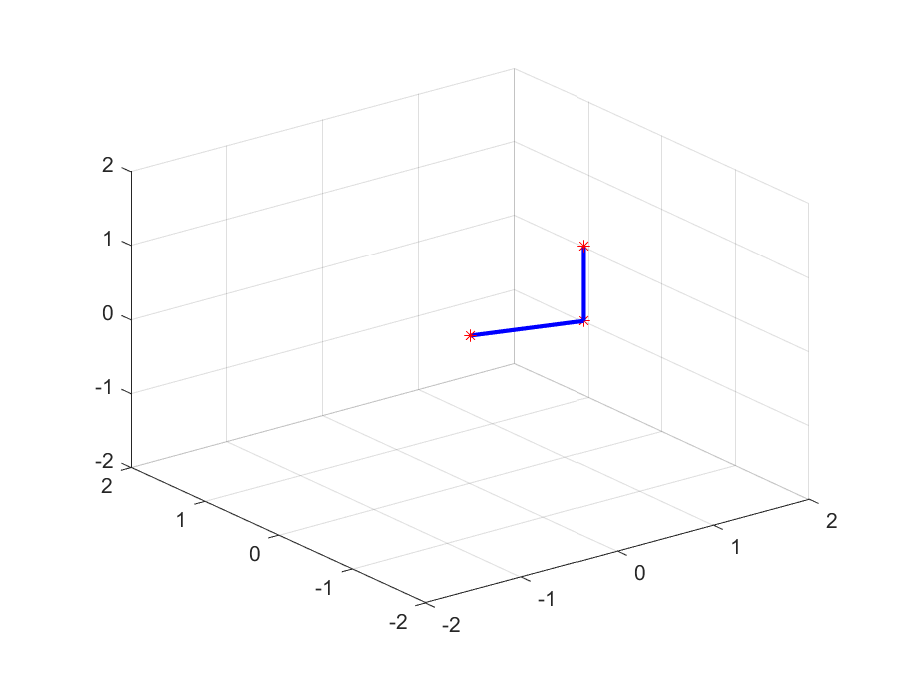
\includegraphics [width=4in]{main_06.eps}


\subsection*{d) poles}

\begin{par}
Checking the poles with pzplot() and pole():
\end{par} \vspace{1em}
\begin{verbatim}
close;
pzplot(H);
pole(sys_ss)
\end{verbatim}

        \color{lightgray} \begin{verbatim}
ans =

         0
         0
   27.9643
  -27.9643

\end{verbatim} \color{black}
    
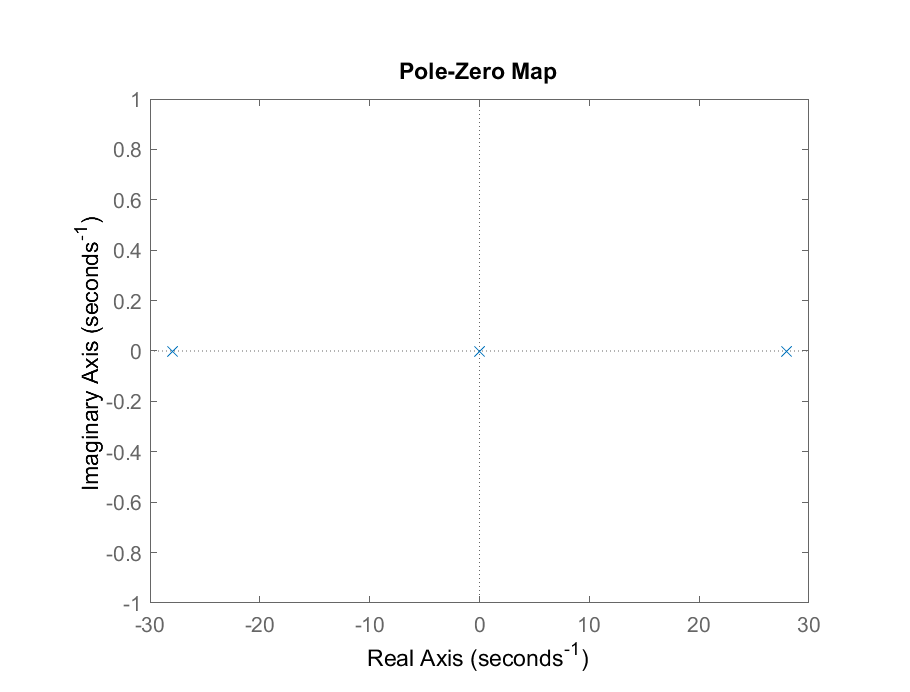
\includegraphics [width=4in]{main_07.eps}
\begin{par}
Our system has four poles:
\end{par} \vspace{1em}
\begin{par}
$$ \left[0, 0, 27.9643, -27.9643 \right]$$
\end{par} \vspace{1em}
\begin{par}
The system has poles in the right half-plane, and is therefore unstable.
\end{par} \vspace{1em}
\begin{verbatim}
close;

%%e) Feedback gain vector
% We need to find a gain vector $\vec{k} = [k_1, k_2, k_3, k_4]$ Which brings the poles/eigenvalues to -10, for our system:
\end{verbatim}
\begin{par}
$$\dot{\vec{x}} = A\vec{x} + \vec{B}T$$
\end{par} \vspace{1em}
\begin{par}
We can do this by using the acker() commands, specifying our desired pole locations
\end{par} \vspace{1em}
\begin{verbatim}
P = [-10, -10, -10, -10];
K = acker(A, B, P)
A_CL = A-B*K;
\end{verbatim}

        \color{lightgray} \begin{verbatim}
K =

   -0.0522    0.4896   -0.0209    0.0203

\end{verbatim} \color{black}
    

\subsection*{f) new A matrix}

\begin{par}
We have found a K matrix/vector such that the poles of our new system is stable (this requires full state estimation). We did this by implicitly defining our control input $T$ as: $$ T = r-\vec{k}\vec{x} $$
\end{par} \vspace{1em}
\begin{par}
Where $r$ is the reference/input. In this way, our new system becomes:
\end{par} \vspace{1em}
\begin{par}
$$ \dot{\vec{x}} = A\vec{x} + B(r-\vec{k}\vec{x}) $$
\end{par} \vspace{1em}
\begin{par}
$$ \dot{\vec{x}} = A\vec{x} + Br-B\vec{k}\vec{x} $$
\end{par} \vspace{1em}
\begin{par}
$$ \dot{\vec{x}} = (A-B\vec{k})\vec{x} + Br $$
\end{par} \vspace{1em}
\begin{par}
We now arrive at a new state space representation of our system, by defining our modified A-matrix $A_{CL}$:
\end{par} \vspace{1em}
\begin{par}
$$ A_{CL} = (A-B\vec{k})$$
\end{par} \vspace{1em}
\begin{par}
$$ \dot{\vec{x}} = A_{CL}\vec{x} + Br $$
\end{par} \vspace{1em}
\begin{par}
$$ \vec{y} = C\vec{x} $$
\end{par} \vspace{1em}
\begin{verbatim}
A_CL
\end{verbatim}

        \color{lightgray} \begin{verbatim}
A_CL =

         0         0    1.0000         0
         0         0         0    1.0000
   48.0887 -269.9112   19.2355  -18.6771
  152.5159 -648.0887   61.0064  -59.2355

\end{verbatim} \color{black}
    

\subsection*{g) step responses}

\begin{verbatim}
new_sys = ss(A_CL, B, C, D);
\end{verbatim}
\begin{verbatim}
close;
step(new_sys);
\end{verbatim}

\includegraphics [width=4in]{main_08.eps}



\end{document}

